% =====================================================================
%  Photosynthesis Inquiry Sheet — Grade 11 American Program Biology
%  Al-Hayat International School, Aramoun, Lebanon
%  Compile with XeLaTeX (twice). Needs the Inter font and his-logo.png
%  in the same folder. Minimum font size: 12 pt.
% =====================================================================
\documentclass[12pt,a4paper]{article}
\usepackage[a4paper,top=1.6cm,bottom=1.7cm,left=1.7cm,right=1.7cm,headheight=34pt,headsep=12pt]{geometry}
\usepackage{fontspec}
\setmainfont{Inter}[BoldFont={Inter SemiBold}]
\newfontfamily\display{Inter Display}[BoldFont={Inter Display Bold}]
\usepackage{amsmath}
\usepackage[table]{xcolor}
\usepackage{graphicx,tikz,pgfplots,enumitem,array,tabularx,fancyhdr,lastpage,needspace}
\usepackage[most]{tcolorbox}
\usetikzlibrary{arrows.meta,decorations.pathmorphing,positioning,calc,shapes.geometric}
\pgfplotsset{compat=1.18}

% ---------- colours sampled from the HIS logo ----------
\definecolor{navy}{HTML}{0A4F8F}
\definecolor{hisblue}{HTML}{0068B0}
\definecolor{hissky}{HTML}{00B0E0}
\definecolor{hisgold}{HTML}{F8D000}
\definecolor{hisred}{HTML}{F2361C}
\definecolor{leaf}{HTML}{2E8B47}
\definecolor{leafsoft}{HTML}{E3F3E7}
\definecolor{lr}{HTML}{9A7100}
\definecolor{lrsoft}{HTML}{FFF6CF}
\definecolor{drsoft}{HTML}{E1F0FB}
\definecolor{rose}{HTML}{D8321A}
\definecolor{rosesoft}{HTML}{FDEAE6}
\definecolor{thyl}{HTML}{7CC48C}
\definecolor{thylin}{HTML}{D9F1DD}
\definecolor{stroma}{HTML}{CDE8F8}
\definecolor{muted}{HTML}{4E6176}
% molecules (same colours as the web page)
\definecolor{cwater}{HTML}{0FA3D8}\definecolor{csun}{HTML}{F5B800}\definecolor{cadp}{HTML}{E25B2B}
\definecolor{catp}{HTML}{F2361C}\definecolor{cnadp}{HTML}{8A63D2}\definecolor{cnadph}{HTML}{6A3FC0}
\definecolor{co}{HTML}{25A7A0}\definecolor{cco}{HTML}{5B6B7C}\definecolor{cglu}{HTML}{2E8B47}

\setlength{\parindent}{0pt}\setlength{\parskip}{5pt}\linespread{1.12}
\setlist{itemsep=2pt,topsep=2pt}

% ---------- header / footer ----------
\pagestyle{fancy}\fancyhf{}
\renewcommand{\headrule}{\hbox to\headwidth{\color{hisred}\leaders\hrule height 1.4pt\hskip0.25\headwidth\color{hisgold}\leaders\hrule height 1.4pt\hskip0.25\headwidth\color{hissky}\leaders\hrule height 1.4pt\hskip0.25\headwidth\color{hisblue}\leaders\hrule height 1.4pt\hfill}}
\fancyhead[L]{\raisebox{-0.32\height}{
\includegraphics[height=0.95cm]{his-logo.png}}\hspace{6pt}\color{navy}\textbf{Al-Hayat International School}}
\fancyhead[R]{\color{muted}Grade 11 AP Biology · Photosynthesis}
\fancyfoot[C]{\color{muted}Page \thepage\ of \pageref{LastPage}}
\fancypagestyle{first}{\fancyhf{}\renewcommand{\headrule}{}\fancyfoot[C]{\color{muted}Page \thepage\ of \pageref{LastPage}}}

% ---------- building blocks ----------
\newcommand{\partbanner}[3]{\par\needspace{5\baselineskip}\vspace{4pt}\noindent\begin{tikzpicture}
  \node[fill=#1,text=white,rounded corners=10pt,inner sep=6pt,font=\bfseries] (b) {#2};
  \node[right=8pt of b,font=\display\bfseries\LARGE,text=navy] {#3};\end{tikzpicture}\par\vspace{0pt}}
\newcommand{\sect}[1]{\par\needspace{8\baselineskip}\vspace{4pt}{\display\bfseries\Large\color{navy}#1}\par\vspace{0pt}}
\newcommand{\Q}[1]{\textbf{\color{hisblue}#1}\ }
\newcommand{\blank}[1][3cm]{\rule[-2pt]{#1}{0.6pt}}
\newcommand{\answerlines}[1]{\par\vspace{0pt}\begin{tikzpicture}
  \foreach \i in {1,...,#1}{\draw[muted!45] (0,-\i*0.92) -- (\linewidth-0.4pt,-\i*0.92);}
  \path (0,0) (0,-#1*0.92-0.12);\end{tikzpicture}\par}
\newcommand{\checkbox}{\tikz[baseline=-3pt]\draw[muted,line width=0.8pt,rounded corners=1.5pt] (0,-0.17) rectangle (0.38,0.21);}
\newcommand{\numbox}{\tikz[baseline=-4pt]\draw[muted,line width=0.9pt,rounded corners=2pt] (0,-0.25) rectangle (0.75,0.32);}
\newcommand{\mol}[2]{\textcolor{#1}{\textbf{#2}}}

\tcbset{base/.style={enhanced,boxrule=0pt,leftrule=5pt,arc=6pt,left=10pt,right=10pt,top=5pt,bottom=5pt,
        fonttitle=\bfseries,coltitle=#1,attach title to upper={\ }}}
\newtcolorbox{hook}[1][]{base=lr,colback=lrsoft,colframe=hisgold!90!black,title={#1}}
\newtcolorbox{teaser}[1][]{base=rose,colback=rosesoft,colframe=rose,title={#1}}
\newtcolorbox{real}[1][]{base=leaf,colback=leafsoft,colframe=leaf,title={#1}}

\tikzset{
  tok/.style={rounded corners=8pt,text=white,font=\bfseries,inner xsep=7pt,inner ysep=4pt},
  arr/.style={-{Latex[length=3mm]},line width=1.6pt},
  disc/.style={fill=thyl,draw=leaf,rounded corners=4pt}}
\newcommand{\granum}[5]{% x y width discs gap
  \foreach \k in {1,...,#4}{\filldraw[disc] (#1,{#2-(\k-1)*#5}) rectangle ++(#3,-0.9*#5);}}

\begin{document}
\thispagestyle{first}

% ===================== TITLE =====================
\begin{tcolorbox}[enhanced,colback=navy,colframe=navy,arc=10pt,left=12pt,right=12pt,top=10pt,bottom=10pt,
  interior style={left color=navy!90!black,right color=hissky}]
\color{white}
\begin{tabular}{@{}m{3.0cm}@{}m{13cm}@{}}
\tikz\node[fill=white,rounded corners=8pt,inner sep=4pt]{
\includegraphics[height=2.3cm]{his-logo.png}}; &
{\bfseries\large Al-Hayat International School}\newline Aramoun, Mount Lebanon · American High School Program\par\vspace{6pt}
{\display\bfseries\fontsize{21}{25}\selectfont Photosynthesis: Following the Energy}\par\vspace{2pt}
Biology · Grade 11 AP · Student Inquiry Sheet\\
\end{tabular}
\end{tcolorbox}
\vspace{-8pt}\noindent\tikz{\foreach \c [count=\i from 0] in {hisred,hisgold,hissky,hisblue}{\fill[\c] (\i*0.25*\linewidth,0) rectangle ++(0.25*\linewidth,0.14);}}\par
\begin{tabularx}{\linewidth}{@{}l X l p{2.8cm} l p{2.8cm}@{}}
\textbf{Name:} & \hrulefill & \textbf{Section:} & \hrulefill & \textbf{Date:} & \hrulefill
\end{tabularx}

\begin{hook}[The Bekaa greenhouse.]
In January, Rami's tomatoes in his greenhouse near Zahleh grow slowly. The days are short and cloudy. He wonders whether to switch on lamps over his plants. By the end of today you will advise him.
\end{hook}
\Q{Q0. Gut feeling.} Will the lamps help? Write your first guess.
\answerlines{2}

\sect{The whole story in one line}
\[\text{6\,CO}_2 + \text{6\,H}_2\text{O}\ \xrightarrow[\text{\normalsize chlorophyll}]{\text{\normalsize light energy}}\ \text{C}_6\text{H}_{12}\text{O}_6 + \text{6\,O}_2\]
\centerline{carbon dioxide + water $\longrightarrow$ glucose + oxygen}
A plant does this in two linked stages inside the chloroplast: the \mol{lr}{light reaction} and the \mol{hisblue}{dark reaction}.

% ===================== PART 1 =====================
\partbanner{lr}{Part 1}{The light reaction}
The light-dependent reaction captures the energy of sunlight and stores it in two energy carriers: \mol{catp}{ATP} and \mol{cnadph}{NADPH}.

\sect{1.1 Location: thylakoids and grana}
\begin{center}
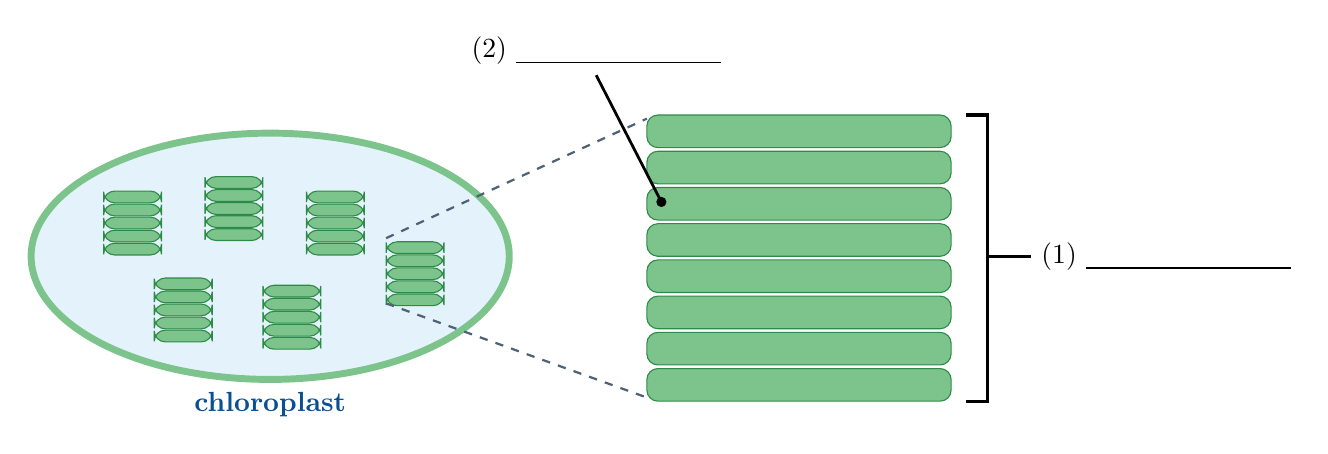
\begin{tikzpicture}[scale=0.92]
  % chloroplast
  \filldraw[fill=stroma!55,draw=thyl,line width=2.5pt] (0,0) ellipse (3.3 and 1.7);
  \foreach \x/\y in {-2.3/0.9,-0.9/1.1,0.5/0.9,1.6/0.2,-1.6/-0.3,-0.1/-0.4}{\granum{\x}{\y}{0.8}{5}{0.18}}
  \node[font=\bfseries,text=navy] at (0,-2.05) {chloroplast};
  % zoom lines
  \draw[muted,dashed,line width=0.8pt] (1.6,0.25) -- (5.2,1.9);
  \draw[muted,dashed,line width=0.8pt] (1.6,-0.65) -- (5.2,-1.95);
  % big granum
  \granum{5.2}{1.95}{4.2}{8}{0.5}
  \draw[line width=1.2pt] (9.6,1.95) -- (9.9,1.95) -- (9.9,-2.0) -- (9.6,-2.0);
  \draw[line width=1pt] (9.9,0) -- (10.5,0) node[right] {(1) \blank[2.6cm]};
  \draw[line width=1pt] (5.4,0.75) -- (4.5,2.5) node[above] {(2) \blank[2.6cm]};
  \fill (5.4,0.75) circle (2pt);
\end{tikzpicture}
\end{center}

\Q{Q1.} Label the diagram. Use the words \textbf{granum} and \textbf{thylakoid}.

\Q{Q2.} The light reaction takes place in the \blank[3.4cm] membranes, which are stacked into \blank[3.4cm]\,.

\begin{teaser}[Q3. Brain teaser:]
Why do you think a chloroplast has its thylakoids \emph{stacked} into many grana instead of having just one big thylakoid?
\answerlines{2}
\end{teaser}

\sect{1.2 Steps of the light reaction}
\begin{center}
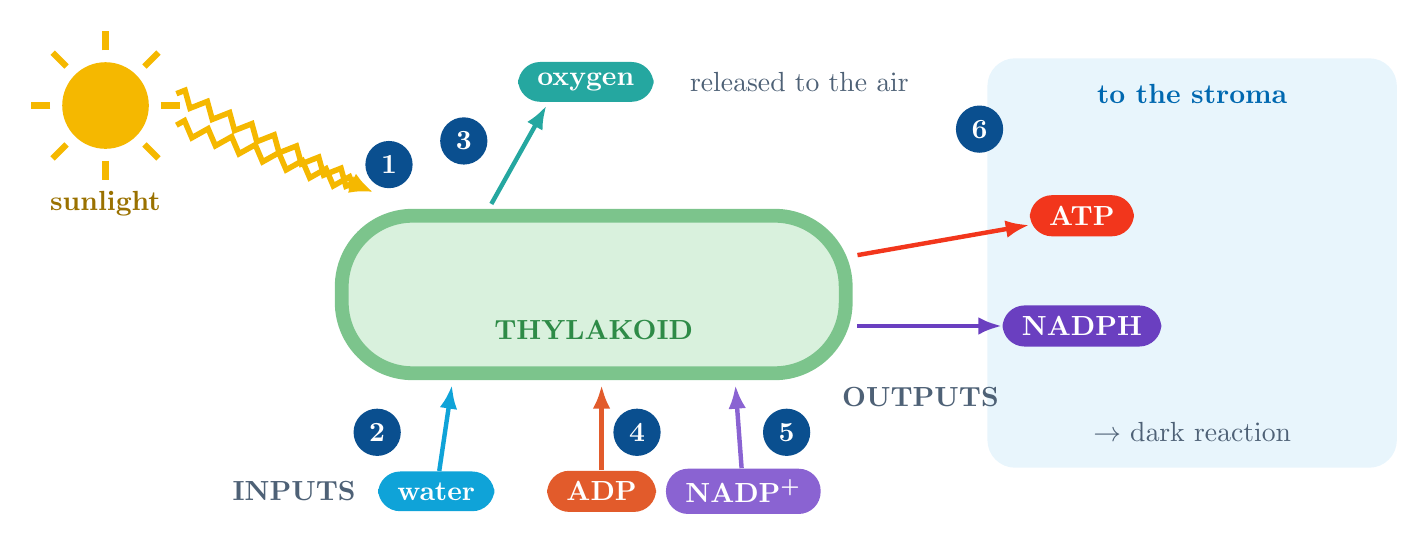
\begin{tikzpicture}[x=1cm,y=1cm]
  \fill[stroma!45,rounded corners=10pt] (12.2,0.4) rectangle (17.4,5.6);
  \node[text=hisblue,font=\bfseries,align=center] at (14.8,5.15) {to the stroma};
  \node[text=muted,align=center] at (14.8,0.85) {$\rightarrow$ dark reaction};
  % sun
  \fill[csun] (1.0,5.0) circle (0.55);
  \foreach \a in {0,45,...,315}{\draw[csun,line width=2.2pt] ($(1.0,5.0)+(\a:0.7)$) -- ($(1.0,5.0)+(\a:0.95)$);}
  \node[text=lr,font=\bfseries] at (1.0,3.75) {sunlight};
  \foreach \yy in {4.75,5.15}{\draw[csun,line width=2pt,-{Latex[length=3mm]},decorate,decoration={zigzag,segment length=9pt,amplitude=2.5pt,post length=6pt}] (1.9,\yy) -- (4.4,3.9);}
  % thylakoid
  \filldraw[fill=thylin,draw=thyl,line width=5pt,rounded corners=0.9cm] (4.0,1.6) rectangle (10.4,3.6);
  \node[text=leaf,font=\bfseries] at (7.2,2.15) {THYLAKOID};
  \node[circle,fill=navy,text=white,font=\bfseries,inner sep=1.5pt,minimum size=0.6cm] at (4.6,4.25) {1};
  % inputs from bottom
  \node[tok,fill=cwater] (w) at (5.2,0.1) {water};
  \node[tok,fill=cadp] (a) at (7.3,0.1) {ADP};
  \node[tok,fill=cnadp] (n) at (9.1,0.1) {NADP\textsuperscript{+}};
  \draw[arr,cwater] (w) -- (5.4,1.45); \draw[arr,cadp] (a) -- (7.3,1.45); \draw[arr,cnadp] (n) -- (9.0,1.45);
  \node[text=muted,font=\bfseries,anchor=east] at (4.3,0.1) {INPUTS};
  % oxygen out
  \draw[arr,co] (5.9,3.75) -- (6.6,5.0);
  \node[tok,fill=co] at (7.1,5.3) {oxygen};
  \node[text=muted,anchor=west] at (8.3,5.3) {released to the air};
  % ATP NADPH out
  \node[tok,fill=catp] (atp) at (13.4,3.6) {ATP};
  \node[tok,fill=cnadph] (nadph) at (13.4,2.2) {NADPH};
  \draw[arr,catp] (10.55,3.1) -- (atp); \draw[arr,cnadph] (10.55,2.2) -- (nadph);
  \node[text=muted,font=\bfseries] at (11.35,1.3) {OUTPUTS};
  % markers
  \foreach \lab/\x/\y in {2/4.45/0.85,3/5.55/4.55,4/7.75/0.85,5/9.65/0.85,6/12.1/4.7}{
    \node[circle,fill=navy,text=white,font=\bfseries,inner sep=1.5pt,minimum size=0.6cm] at (\x,\y) {\lab};}
\end{tikzpicture}
\end{center}

\Q{Q4.} Number the steps 1--6 in the order they happen. The numbers on the diagram will help.

\renewcommand{\arraystretch}{1.25}
\begin{tabularx}{\linewidth}{@{}p{1.2cm} X@{}}
\numbox & \mol{cadp}{ADP} is charged up to make \mol{catp}{ATP}. \\
\numbox & \mol{co}{Oxygen} from the water is released into the air. \\
\numbox & ATP and NADPH carry the energy to the stroma, for the dark reaction. \\
\numbox & Chlorophyll in the thylakoid membrane absorbs \mol{lr}{sunlight}. \\
\numbox & \mol{cnadp}{NADP\textsuperscript{+}} is loaded up to make \mol{cnadph}{NADPH}. \\
\numbox & The light energy is used to split \mol{cwater}{water}. \\
\end{tabularx}

\sect{1.3 The reaction}
\Q{Q5.} Complete the light reaction.
\[\text{water} \;+\; \underline{\hspace{2.8cm}} \;+\; \text{ADP} \;+\; \underline{\hspace{2.4cm}}\ \xrightarrow{\text{\normalsize in thylakoids}}\ \underline{\hspace{2.6cm}} \;+\; \text{ATP} \;+\; \underline{\hspace{2.4cm}}\]

\sect{1.4 Inputs and outputs}
\Q{Q6.} Tick one box for each molecule in the \textbf{light reaction}.
\begin{center}
\renewcommand{\arraystretch}{1.3}
\begin{tabular}{|l|*{7}{>{\centering\arraybackslash}p{1.55cm}|}}
\hline
\rowcolor{lrsoft} & \textbf{water} & \textbf{sunlight} & \textbf{ADP} & \textbf{NADP\textsuperscript{+}} & \textbf{oxygen} & \textbf{ATP} & \textbf{NADPH}\\\hline
\textbf{Input}  & \checkbox & \checkbox & \checkbox & \checkbox & \checkbox & \checkbox & \checkbox \\\hline
\textbf{Output} & \checkbox & \checkbox & \checkbox & \checkbox & \checkbox & \checkbox & \checkbox \\\hline
\end{tabular}
\end{center}

\begin{teaser}[Q7. Brain teaser:]
Every breath you take contains oxygen made by plants. Look at the inputs: which molecule does that oxygen come from?
\answerlines{1}
\end{teaser}

\sect{1.5 Effect of sunlight intensity}
A pondweed is placed under a lamp. The \textbf{oxygen bubbles} it gives off show how fast the light reaction runs.
\begin{center}
\renewcommand{\arraystretch}{1.35}
\begin{tabular}{|l|*{6}{>{\centering\arraybackslash}p{1.15cm}|}}
\hline
\rowcolor{lrsoft}\textbf{Light intensity (\%)} & 0 & 20 & 40 & 60 & 80 & 100\\\hline
\textbf{O\textsubscript{2} bubbles per minute} & 0 & 15 & 23 & 26 & 28 & 29\\\hline
\end{tabular}
\end{center}
\Q{Q8.} Plot the data and join the points with a smooth curve.
\begin{center}
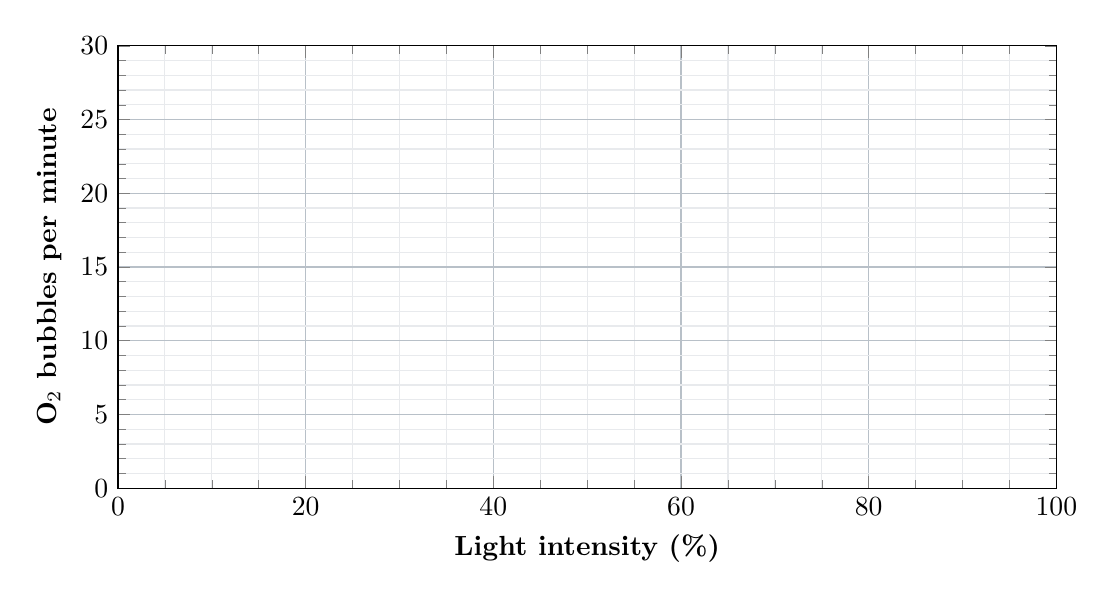
\begin{tikzpicture}
\begin{axis}[width=13.5cm,height=7.2cm,xmin=0,xmax=100,ymin=0,ymax=30,
  xtick={0,20,...,100},ytick={0,5,...,30},minor x tick num=3,minor y tick num=4,
  grid=both,major grid style={muted!40},minor grid style={muted!13},
  xlabel={Light intensity (\%)},ylabel={O$_2$ bubbles per minute},
  tick label style={font=\normalsize},label style={font=\normalsize\bfseries}]
\addplot[draw=none] coordinates {(0,0)};
\end{axis}
\end{tikzpicture}
\end{center}

\Q{Q9.} Describe what happens to the rate as light intensity increases.
\answerlines{2}

\begin{teaser}[Q10. Brain teaser:]
Between 80\% and 100\% light, the plant gets more light but hardly makes more oxygen. Suggest why.
\answerlines{2}
\end{teaser}

\begin{real}[Q11. Real world:]
Use your graph to explain why Rami's tomatoes grow slowly on short, cloudy January days.
\answerlines{2}
\end{real}

% ===================== PART 2 =====================
\partbanner{hisblue}{Part 2}{The dark reaction}
The light-independent reaction (Calvin cycle) uses the energy in \mol{catp}{ATP} and \mol{cnadph}{NADPH} to build \mol{cglu}{glucose} from \mol{cco}{carbon dioxide}.

\sect{2.1 Location: the stroma}
\begin{minipage}[c]{0.46\linewidth}
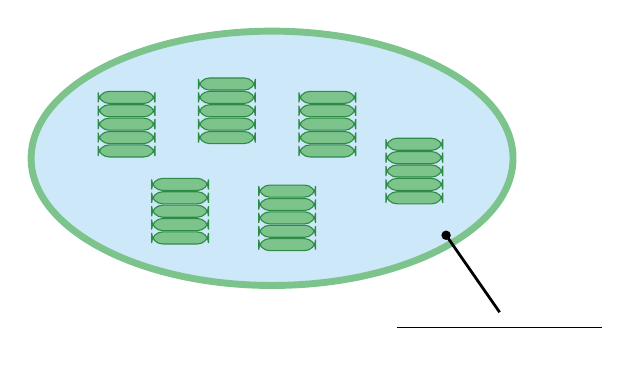
\begin{tikzpicture}[scale=0.85]
  \filldraw[fill=stroma,draw=thyl,line width=2.5pt] (0,0) ellipse (3.6 and 1.9);
  \foreach \x/\y in {-2.6/1.0,-1.1/1.2,0.4/1.0,1.7/0.3,-1.8/-0.3,-0.2/-0.4}{\granum{\x}{\y}{0.85}{5}{0.2}}
  \draw[line width=1pt] (2.6,-1.15) -- (3.4,-2.3) node[below] {\blank[2.6cm]};
  \fill (2.6,-1.15) circle (2pt);
\end{tikzpicture}
\end{minipage}\hfill
\begin{minipage}[c]{0.5\linewidth}
\Q{Q12.} The dark reaction takes place in the \blank[3cm] of the chloroplast. Label it on the diagram.

\Q{Q13.} Why is it useful that the stroma surrounds the thylakoids?
\answerlines{3}
\end{minipage}

\sect{2.2 Steps of the dark reaction}
\begin{center}
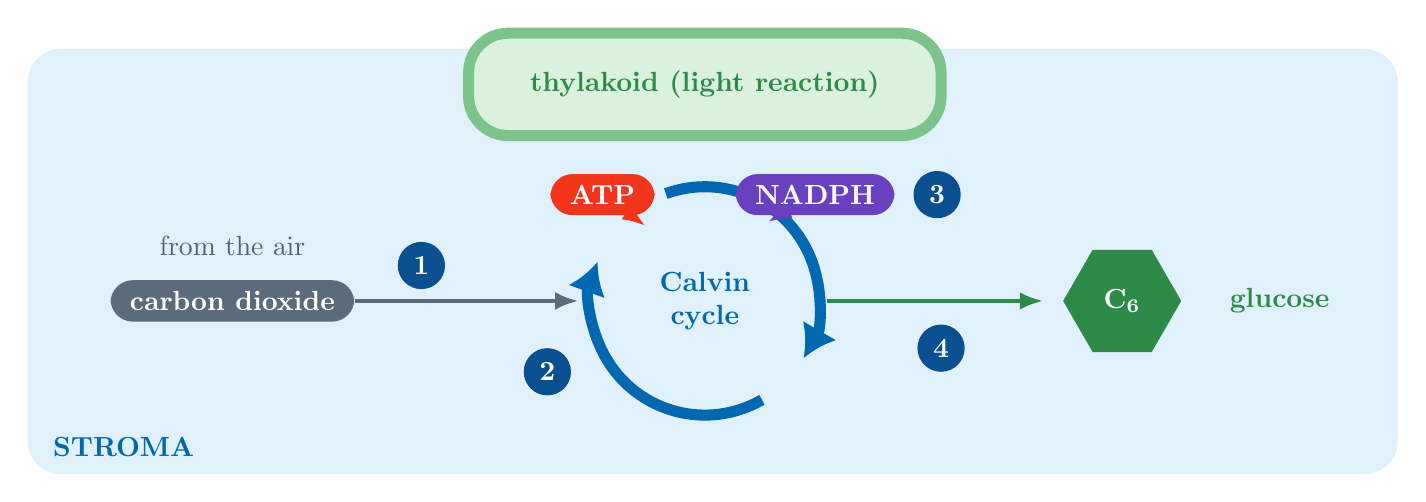
\begin{tikzpicture}[x=1cm,y=1cm]
  \fill[stroma!60,rounded corners=12pt] (0,0) rectangle (17.4,5.4);
  \node[text=hisblue,font=\bfseries,anchor=south west] at (0.2,0.1) {STROMA};
  \filldraw[fill=thylin,draw=thyl,line width=4pt,rounded corners=0.5cm] (5.6,4.3) rectangle (11.6,5.6);
  \node[text=leaf,font=\bfseries] at (8.6,4.95) {thylakoid (light reaction)};
  % cycle
  \draw[hisblue,line width=4pt,-{Latex[length=4mm,width=5mm]}] (8.6,2.2) ++(110:1.45) arc (110:-30:1.45);
  \draw[hisblue,line width=4pt,-{Latex[length=4mm,width=5mm]}] (8.6,2.2) ++(-60:1.45) arc (-60:-200:1.45);
  \node[text=hisblue,font=\bfseries,align=center] at (8.6,2.2) {Calvin\\cycle};
  % inputs
  \node[tok,fill=cco] (c) at (2.6,2.2) {carbon dioxide};
  \draw[arr,cco] (c) -- (7.0,2.2);
  \node[text=muted,anchor=south] at (2.6,2.65) {from the air};
  \node[tok,fill=catp] (a) at (7.3,3.55) {ATP};
  \node[tok,fill=cnadph] (n) at (10.0,3.55) {NADPH};
  \draw[arr,catp] (a) -- (7.85,3.15); \draw[arr,cnadph] (n) -- (9.4,3.2);
  % output
  \draw[arr,cglu] (10.15,2.2) -- (12.9,2.2);
  \node[regular polygon,regular polygon sides=6,fill=cglu,minimum size=1.5cm,text=white,font=\bfseries] at (13.9,2.2) {C\textsubscript{6}};
  \node[text=cglu,font=\bfseries] at (15.9,2.2) {glucose};
  \node[circle,fill=navy,text=white,font=\bfseries,inner sep=1.5pt,minimum size=0.6cm] at (5.0,2.65) {1};
  \node[circle,fill=navy,text=white,font=\bfseries,inner sep=1.5pt,minimum size=0.6cm] at (6.6,1.3) {2};
  \node[circle,fill=navy,text=white,font=\bfseries,inner sep=1.5pt,minimum size=0.6cm] at (11.55,3.55) {3};
  \node[circle,fill=navy,text=white,font=\bfseries,inner sep=1.5pt,minimum size=0.6cm] at (11.6,1.6) {4};
\end{tikzpicture}
\end{center}

\Q{Q14.} Number the steps 1--4 in the order they happen.

\begin{tabularx}{\linewidth}{@{}p{1.2cm} X@{}}
\numbox & \mol{catp}{ATP} and \mol{cnadph}{NADPH} supply the energy to build sugar. \\
\numbox & \mol{cglu}{Glucose} is made. The plant uses it or stores it as starch. \\
\numbox & \mol{cco}{Carbon dioxide} from the air enters the stroma. \\
\numbox & CO\textsubscript{2} is fixed (joined) into the Calvin cycle. \\
\end{tabularx}

\sect{2.3 The reaction}
\Q{Q15.} Complete the dark reaction.
\[\underline{\hspace{3.4cm}} \;+\; \text{ATP} \;+\; \underline{\hspace{2.6cm}}\ \xrightarrow{\text{\normalsize in stroma}}\ \underline{\hspace{3cm}}\]

\sect{2.4 Inputs and outputs}
\Q{Q16.} Tick one box for each molecule in the \textbf{dark reaction}.
\begin{center}
\renewcommand{\arraystretch}{1.3}
\begin{tabular}{|l|*{4}{>{\centering\arraybackslash}p{2.9cm}|}}
\hline
\rowcolor{drsoft} & \textbf{carbon dioxide} & \textbf{ATP} & \textbf{NADPH} & \textbf{glucose}\\\hline
\textbf{Input}  & \checkbox & \checkbox & \checkbox & \checkbox \\\hline
\textbf{Output} & \checkbox & \checkbox & \checkbox & \checkbox \\\hline
\end{tabular}
\end{center}

\begin{teaser}[Q17. Brain teaser:]
The dark reaction does not use light directly. So does it keep making glucose all night long? Explain.
\answerlines{2}
\end{teaser}

\sect{2.5 Effect of available energy}
A plant is kept in bright light. At minute 5 the lights are switched off.
\begin{center}
\renewcommand{\arraystretch}{1.35}
\begin{tabular}{|l|*{11}{>{\centering\arraybackslash}p{0.62cm}|}}
\hline
\rowcolor{drsoft}\textbf{Time (min)} & 0 & 1 & 2 & 3 & 4 & 5 & 6 & 7 & 8 & 9 & 10\\\hline
\textbf{Glucose made (units/min)} & 12 & 12 & 12 & 12 & 12 & 12 & 6 & 2 & 0 & 0 & 0\\\hline
\end{tabular}
\end{center}
\Q{Q18.} Plot the data. What happens to glucose production after the light goes off?
\begin{center}
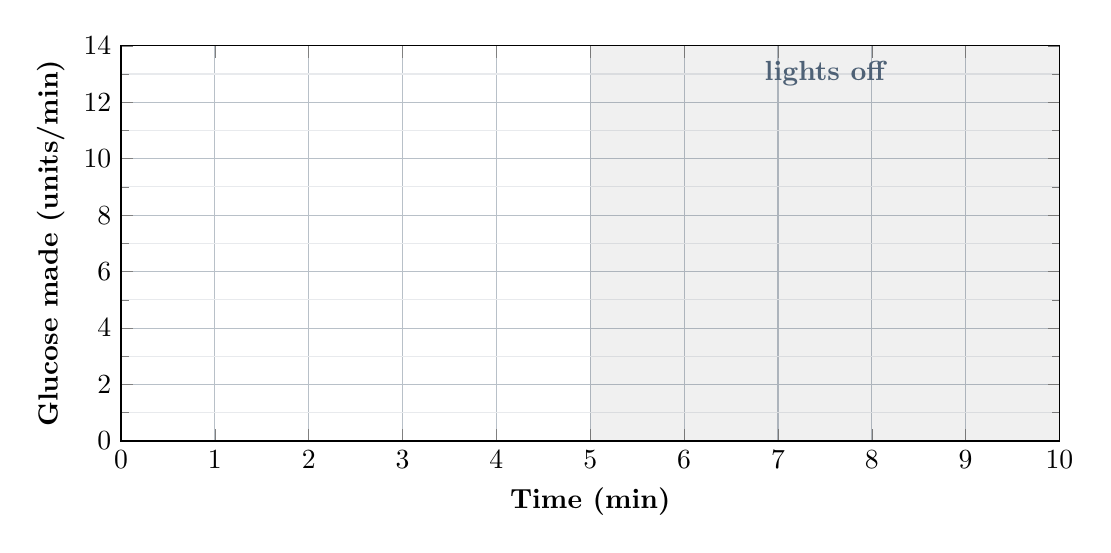
\begin{tikzpicture}
\begin{axis}[width=13.5cm,height=6.6cm,xmin=0,xmax=10,ymin=0,ymax=14,
  xtick={0,1,...,10},ytick={0,2,...,14},minor y tick num=1,
  grid=both,major grid style={muted!40},minor grid style={muted!13},
  xlabel={Time (min)},ylabel={Glucose made (units/min)},
  tick label style={font=\normalsize},label style={font=\normalsize\bfseries}]
\fill[black,opacity=.06] (axis cs:5,0) rectangle (axis cs:10,14);
\node[font=\normalsize\bfseries,text=muted] at (axis cs:7.5,13) {lights off};
\addplot[draw=none] coordinates {(0,0)};
\end{axis}
\end{tikzpicture}
\end{center}
\answerlines{1}

\Q{Q19.} Explain why glucose production stops, even though carbon dioxide is still available.
\answerlines{2}

\begin{teaser}[Q20. Brain teaser:]
Predict what happens if a plant gets \emph{more} ATP and NADPH than usual. Will glucose production rise forever?
\answerlines{2}
\end{teaser}

% ===================== PART 3 =====================
\partbanner{leaf}{Part 3}{Connect the two reactions}
\begin{center}
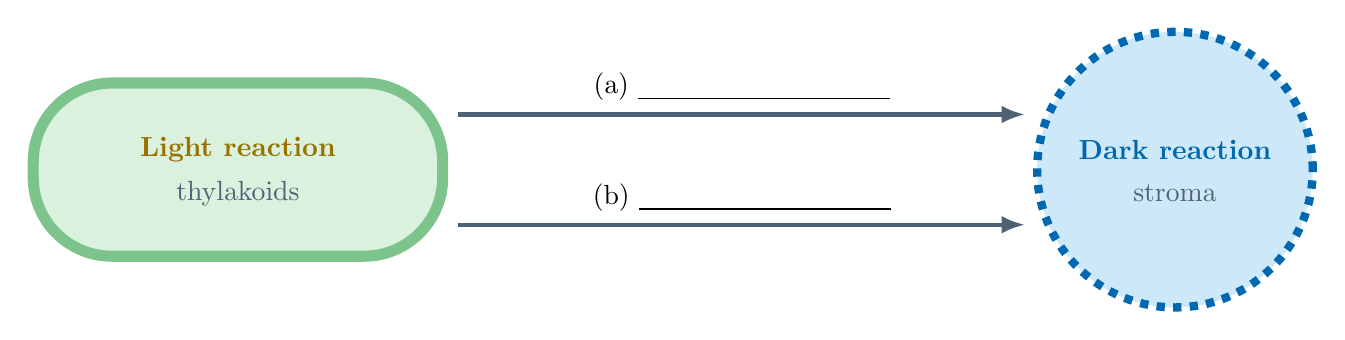
\begin{tikzpicture}[x=1cm,y=1cm]
  \filldraw[fill=thylin,draw=thyl,line width=4pt,rounded corners=1cm] (0.4,0.4) rectangle (5.6,2.6);
  \node[text=lr,font=\bfseries] at (3,1.75) {Light reaction};\node[text=muted] at (3,1.2) {thylakoids};
  \filldraw[fill=stroma,draw=hisblue,line width=3pt,dashed] (14.9,1.5) circle (1.75);
  \node[text=hisblue,font=\bfseries] at (14.9,1.75) {Dark reaction};\node[text=muted] at (14.9,1.2) {stroma};
  \draw[arr,muted] (5.8,2.2) -- (13.0,2.2); \draw[arr,muted] (5.8,0.8) -- (13.0,0.8);
  \node[above] at (9.4,2.25) {(a) \blank[3.2cm]}; \node[above] at (9.4,0.85) {(b) \blank[3.2cm]};
\end{tikzpicture}
\end{center}
\Q{Q21.} Write the two molecules that carry energy from the light reaction to the dark reaction on the arrows.

\begin{real}[Q22. Advise Rami (Claim -- Evidence -- Reasoning).]
Should Rami switch on lamps over his tomatoes on cloudy January days? Use your graph from 1.5 as evidence, and explain using both reactions.

\textbf{Claim:}\answerlines{1}
\textbf{Evidence:}\answerlines{2}
\textbf{Reasoning:}\answerlines{4}
\end{real}

\Q{Q23.} Look back at Q0. Was your gut feeling right? What changed your mind (or confirmed it)?
\answerlines{3}

\sect{Exit ticket · 3 – 2 – 1}
\textbf{3} differences between the light and dark reactions
\answerlines{3}
\textbf{2} molecules that link them \blank[4cm] \quad \blank[4cm]\par
\textbf{1} question you still have
\answerlines{1}

\end{document}
